\title{Lab Three: Introduction to Verilog}
\author{Ben Smith}

%| This is a header file for Latex documents  
%| It contains a number of common packages, settings, and custom macros that I frequently use.
\documentclass[9pt,journal]{IEEEtran}

\usepackage[cmex10]{amsmath}        %| American Mathematical Society package for fancy maths  b
\interdisplaylinepenalty=2500              %| Restores IEEE line spacing after amsmath

%| IEEE Citation package
\usepackage{cite}
\usepackage[section]{placeins}
\usepackage{array}
\usepackage{dblfloatfix}
\usepackage{color}
\usepackage{graphicx}
\usepackage{float}
\usepackage{url}                         %| Improved URL handling
\usepackage{etoolbox}
\usepackage[font=footnotesize]{subcaption}
\usepackage{listings}
\usepackage{fixltx2e}               %| Better tables than for LaTeX 2e
\usepackage{minted}

%| Highlighting for source code listings
\definecolor{mygreen}{rgb}{0,0.6,0}
\definecolor{ltgray}{rgb}{0.93,0.93,0.93}
\definecolor{dkgray}{rgb}{0.5,0.5,0.5}
\definecolor{mymauve}{rgb}{0.58,0,0.82}
\lstset{
  backgroundcolor=\color{ltgray},  % choose the background color; you must add \usepackage{color} or \usepackage{xcolor}
  basicstyle=\scriptsize\ttfamily, % the size of the fonts that are used for the code
  breakatwhitespace=true,         % sets if automatic breaks should only happen at whitespace
  breaklines=true,                 % sets automatic line breaking
  captionpos=b,                    % sets the caption-position to bottom
  commentstyle=\color{mygreen},    % comment style
  deletekeywords={...},            % if you want to delete keywords from the given language
  escapeinside={\%*}{*)},          % if you want to add LaTeX within your code
  extendedchars=true,              % lets you use non-ASCII characters; for 8-bits encodings only, does not work with UTF-8
  frame=single,                    % adds a frame around the code
  keepspaces=true,                 % keeps spaces in text, useful for keeping indentation of code (possibly needs columns=flexible)
  keywordstyle=\color{blue},       % keyword style
  language=SystemVerilog,          % the language of the code(I modified the .sty for systemverilog, found the code on google)
  morekeywords={*,...},            % if you want to add more keywords to the set
  numbers=left,                    % where to put the line-numbers; possible values are (none, left, right)
  numbersep=4pt,                   % how far the line-numbers are from the code
  numberstyle=\tiny\color{dkgray}, % the style that is used for the line-numbers
  rulecolor=\color{black},         % if not set, the frame-color may be changed on line-breaks within not-black text (e.g. comments (green here))
  showspaces=false,                % show spaces everywhere adding particular underscores; it overrides 'showstringspaces'
  showstringspaces=false,          % underline spaces within strings only
  showtabs=false,                  % show tabs within strings adding particular underscores
  stepnumber=2,                    % the step between two line-numbers. If it's 1, each line will be numbered
  stringstyle=\color{mymauve},     % string literal style
  tabsize=2,                       % sets default tabsize to 2 spaces
  title=\lstname                   % show the filename of files included with \lstinputlisting; also try caption instead of title
}

\lstset{keywordstyle=\color{purple}}
\lstset{keywordstyle={[2]\color{purple}} }
\lstset{keywordstyle={[3]\color{magenta}} }
\lstset{keywordstyle={[4]\color{teal} }}
\lstset{keywordstyle={[5]\color{violet!40}} }

% Alter some LaTeX defaults for better treatment of figures:
  % See p.105 of ''TeX Unbound'' for suggested values.
  % See pp. 199-200 of Lamport's ''LaTeX'' book for details.
  %   General parameters, for ALL pages:
  \renewcommand{\topfraction}{0.9}  % max fraction of floats at top
  \renewcommand{\bottomfraction}{0.8} % max fraction of floats at bottom
  %   Parameters for TEXT pages (not float pages):
  \setcounter{topnumber}{2}
  \setcounter{bottomnumber}{2}
  \setcounter{totalnumber}{4}     % 2 may work better
  \setcounter{dbltopnumber}{2}    % for 2-column pages
  \renewcommand{\dbltopfraction}{0.9} % fit big float above 2-col. text
  \renewcommand{\textfraction}{0.07}  % allow minimal text w. figs
  %   Parameters for FLOAT pages (not text pages):
  \renewcommand{\floatpagefraction}{0.7}  % require fuller float pages
  % N.B.: floatpagefraction MUST be less than topfraction !!
  \renewcommand{\dblfloatpagefraction}{0.7} % require fuller float pages

%| Enables PDF metadata, thumbnails, and navigation
\newcommand\MYhyperrefoptions{
  bookmarks=true,
  bookmarksnumbered=true,
  pdfpagemode={UseOutlines},
  plainpages=false,
  pdfpagelabels=true,
  colorlinks=true,
  linkcolor={black},
  citecolor={black},
  urlcolor={blue},
  pdftitle={CPE/EEE 64 Lab},
  pdfsubject={Engineering},                        
  pdfauthor={Ben Smith},
  pdfkeywords={Logic Design, FPGA, Verilog}}                       

%| Calls hyperref package with the options specified above
\usepackage[\MYhyperrefoptions,pdftex]{hyperref}

%| Font settings
\renewcommand{\sfdefault}{phv}
\renewcommand{\rmdefault}{ptm}
\renewcommand{\ttdefault}{pcr}

%| Restores IEEE table formatting after usage of subcaption package
\captionsetup[table]{format=plain,labelformat=simple,justification=centering, labelsep=newline, singlelinecheck=false, textfont={sc}}

%| Required Lab Demo custom function
%| \demo{Name}{Physical deliverable}{Documentation deliverable}{Process}
%| =================================================================================================
%| for boxed text and stuch
\usepackage{fancybox}
\newenvironment{fminipage}%
{\begin{Sbox}\begin{minipage}}%
{\end{minipage}\end{Sbox}\Ovalbox{\TheSbox}}

%| Actual bawx
\newcommand{\demo}[4] {
\vspace{15px}
\begin{centering}
  \begin{fminipage}{.47\textwidth}
    \vspace{3px}
    \centering{\bfseries \large Laboratory Demo: #1}\\*
    \vspace{10px}
    \begin{tabular}{p{1.4cm}  p{6.3cm}}
      %|==Requirements for lab demo==
      \raggedright Specification:                  &#2\\
      \\
      \raggedright  Deliverable:                   &#3\\
      \\
      \raggedright Process :                       &#4\\
    \end{tabular}
  \end{fminipage}
\end{centering}
}

%| Single figure
%| \small{Location}{Caption}{Label}
%| =================================================================================================
\newcommand{\smallfig}[3] {
  \begin{figure}[H]
    \includegraphics[width=.48\textwidth]{#1}
    \caption{#2}
    \label{#3}
  \end{figure}
}

%| Single figure
%| \simpletable{c||c}{Caption}{Label}{content}
%| =================================================================================================
\newcommand{\simpletable}[4] {
  \begin{table}[!t]
    \caption{#2}
    \label{#3}
    \centering
    \begin{tabular}{#1}
      \hline
      #4
    \end{tabular}
  \end{table}
}
\begin{document}

  \maketitle
    \begin{abstract}
      Basic properties of the Verilog and System Verilog hardware descriptive languages are described in this document. The focus is on Behavioral modeling, automated verification and modular design.
    \end{abstract}
  %| =================================================================================================
  %| Introduction
  %| =================================================================================================
  \section{Introduction}
    \IEEEPARstart{L}{ab} two will introduce text based design entry, and in particular, Verilog's behavioral modeling ability. It is a powerful tool that allows the digital designer to abstract themselves from the burdens of structural modeling.  Text based design entry is the Industry standard for digital design. The two most prevalent languages, Verilog and VHDL, are both IEEE standards. In the previous lab,  we used schematic representations of gates to implement a design. Individual gate structures and wired them together to implement the design. This provides a great intuitive explanation of what was built on the FPGA but can become very cumbersome in large designs.  Imagine creating Karnaugh maps for all 72GPIO pins, or better yet the 548 user configurable pins on the Altera's larger FPGA The Stratix\cite{Altera:StratixVDeviceOverview}; this is simply unreasonable! Verilog provides a very concise way to describe the behavior of very large systems. Behavioral modeling allows the use of higher level statements like If and Case statements that can implement complex functionality in only a few lines of HDL. If you don't know what these programming constructs are, don't worry, we will explore them in this lab. The purpose of this lab is to introduce the following concepts:
    \begin{itemize}
      \item Verilog behavioral modeling
      \item Verilog's constant syntax
      \item Verilog behavioral blocks
      \item Testbench assertions
      \item Instantiate a System Verilog module
      \item Use a System Verilog Testbench
      \item Synthesize Verilog code for an FPGA
    \end{itemize}

    \subsection{Included Screencasts}
      \begin{enumerate}
        \item TIME - Verilog Module Anatomy, instantiation, modularity, and parameterization
        \item TIME - Verilog testbench and Modelsim
        \item TIME - Netlist Viewers
      \end{enumerate}
    
    \subsection{Verilog Design Entry}
      Verilog is a powerful way to describe circuits. Logic diagrams like those being used in lecture can become cumbersome in large designs. ``Text based design entry'' can be less prone to error because it is easier to track differences in large designs with a diff tool than a sprawling schematic. Verilog is a text based hardware descriptive language the begun being used in ASIC(Application Specific Integrated Circuit). It is now the language of choice for FPGAs(Field Programmable Gate Array) and CPLDs(Computer Programmable Logic Devices). It is important to note that if you have some programming experience Verilog is superficially similar to many programming languages. Quartus provides a comprehensive solution for testing Verilog and synthesizing it for use on their FPGAs and CPLDs. Altera offers a tutorial very similar to the one used in Lab Two for Verilog design entry instead of the graphical method. The same tutorial that was used in lab one is also written for Verilog design entry, it can be \href{ftp://ftp.altera.com/up/pub/Altera_Material/13.0/Tutorials/Verilog/Quartus_II_Introduction.pdf}{found here} for the interested reader.

    \subsection{Anatomy of a Verilog Module}
      The ``module'' is at the heart of Verilog. Clever design will allow you to create a module that you can reuse many times. These labs will stress design for re-usability as it is the core of efficiency in the workplace.
      \lstinputlisting[caption=Template for System Verilog Modules]{./codesnips/exampleModule.sv} 

      Notice the [7:0] next to the wire declarations. This is a way to declare a ``parallel'' bus. We are just hooking up 7 wires at once. Compare this template to the example constant adder module from the Laboratory Procedure section.
      
      \lstinputlisting[caption=Adder from example code]{./codesnips/AdderExample.sv}

    \subsection{Verilog Modularity}
      One of the most important features of Verilog is it's ability to reuse a design. Reusing code allows you to  rapidly assemble and test new designs. The configurability of the FPGA allows a designer to rapidly prototype a design. Reusing these modules is very similar to how you would reuse code in the workplace to be more productive. You could think of this as the source libraries that would be available at the company that you might work for.

    \subsection{Instantiation of a Verilog module}
      At the core of modular design is the module instantiation. Think of it of plopping a piece of hardware down on a breadboard. You could make a LS7400 Verilog module and every instantiation would be another discrete device just like using a real LS7400 on your breadboard. In Verilog the module name, is the name of the module you are instantiating.
      \lstinputlisting[caption=Template for System Verilog module instantiation]{./codesnips/instantiationTemplate.sv}
    
    \subsection{Parameterization of Verilog modules}
      A Verilog module's parameters allow a module to be reused in a number of different situations. An example would be a variable length shift register. In one application you might need a 32-bit version in another a 64-bit. Building the module in a particular manner will allow a parameter to control the length with the parameter. The parameter and its default value is specified in the Adder Module on line
      \begin{lstlisting}
  parameter constant = 4'b0000;
      \end{lstlisting}
      This is the Value that will be used if the parameter is not specified in the module instantiation. An example of parameter usage when instantiating a new module is below. Anything in angle brackets is something that you will need to replace with the information form your design.
      \lstinputlisting[caption=Paramaterized instantiation example]{./codesnips/ParamaterizedInstantiationTemplate.sv}

      Notice the addition of the \#() before the instance name in the last design. We can see the adder module instantiation in the test bench follows this syntax.
      \lstinputlisting[caption=Instantiation example form the testbench]{./codesnips/AdderInstantiationTemplate.sv}

    \subsection{Test Bench for automated debugging}
      The Verilog language roughly breaks into two halves synthesizable and non-synthesizable. The FPGA synthesis can take a very long time, using a simulator to verify individual modules can be much faster than resynthesizing the entire design. The Testbench also offers a unique ability to check expected outputs. This will ensure your design behaves as expected. We will use a test bench to check the provided Verilog modules are providing the desired operation in part C of the procedure. This simulation should be verified against the known truth table for the logic gate to ensure the module is accurate. Verification is a very important topic in logic design. \footnote{If you are particularly driven to be an expert in programmable logic I highly recommend a series of MOOC courses on debugging taught by Andreas Zeller on debugging. Both classes deal only with Python but the way of thinking is important topic. The classes are \href{https://www.udacity.com/course/cs258}{Automated Software Testing} and \href{https://www.udacity.com/course/cs259}{Software Debugging} the first few videos in each series cover the important topics. Keep in mind these classes are outside the scope of this class and I only offer them because how much they helped me be a better designer.}

      \lstinputlisting[caption=Example testbench]{./codesnips/AdderTestbench.sv}

      This section will explore the basics of Modelsim and using a Verilog Testbench in Modelsim. Start a new simulation and add the waveforms as shown in screencast 2. Figure \ref{LogicOut} shows an example of what the wave section should look like for the example adder. 
      \begin{figure}[H]
        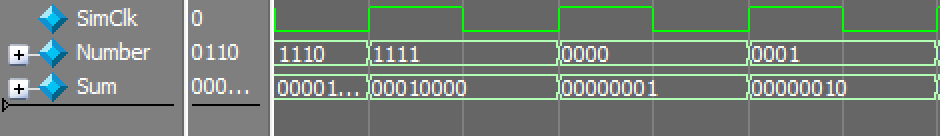
\includegraphics[width=.48\textwidth]{Images/LogicOutput.png}
        \caption{Example output of testbench}
        \label{LogicOut}
      \end{figure}

      Take a moment to look at the simulation transcript, it provides the states of the logic elements being tested.
      I prefer having the simulator give a test listing instead of reading the waveforms. This is from the \$display()
      lines in the testbench. listing the outputs can be a very powerful debugging tool. I typically use the \$assert()
      statement, which will be explored below, which can execute two different blocks of code based on a logical test and alert you when an unexpected result is produced.
      \lstinputlisting[caption=Example output of Testbench]{./codesnips/testbenchoutput.txt}

      Verification is a large part of working with Verilog. Verilog provides little assistance in assuring the functionality of a design. You must catch the flaws in your design. This comes from a through understanding of the specification and through testing to ensure adherance. To ensure this a simulator called Modelsim is used extensively in logic design with Verilog. Fortunately Verilog offers a number of tools to make checking your code easier for use in simulation. The most basic, but very powerful, is the assertion. The assertion will run two different blocks of code depending on if a logical condition is met, It works much like an if statement.
      \lstinputlisting[caption=Template for System Verilog Modules]{./codesnips/AssertionTemplate.sv}

      The same code is used to test the adder from this lab's example code. The true case is used to display the valid output of the module. The false case throws a simulation error and shows the user the case. The syntax used to display text to the console follows ``printf'' syntax popularized by the C language. A reference for use can be found on \href{https://en.wikipedia.org/wiki/Printf_format_string}{Wikipedia}.
      \lstinputlisting[caption=Example assertion from adder testbench]{./codesnips/AssertionFromLab.sv}

      The logical statement in this code block checks to see if the output of the module is equal to the sum of specified constant and Number. Many designers write the test bench from specification in advance of the Verilog module. Testing should be an integral part of Verilog development from the beginning.

      All of the code from this first section is provided in source.zip. There is quite a learning curve to this part, be sure to watch the screen cast which describes the included modules. You will be assigned a constant by the lab instructor that the input number will be added to. This number should be entered as a parameter in the adder module's instantiation as is done in the test bench.

  %| =================================================================================================
  %| Procedure: Verilog Testbench
  %| =================================================================================================
  \section{Laboratory Procedure}
    \IEEEPARstart{T}{he} Lab procedure for this lab is a bit more involved. It is the first interaction with text based entry, Signaltap, and Modelsim. The skills learned are industry applicable, I've used all of these tools and methods while working at a firm developing for Altera FPGAs. It's going to seem very foreign, don't worry, ask a lab instructor any questions you might have we're here to help.

  %| =================================================================================================
  %| Procedure: Verilog Testbench
  %| =================================================================================================
  \subsection{Signal Tap Embedded Logic analyzer}
    The single most valuable debugging tool in Quartus is the Signaltap Logic analyzer. The device is implemented by the on chip logic and transmits information to Quartus over the USB link.  Signaltap provides the state of a signal with respect to time. This is identical to the Simulator waveform but is recorded from the running logic on the FPGA. Once again Altera provides a \href{ftp://ftp.altera.com/up/pub/Altera_Material/13.0/Tutorials/Verilog/SignalTap.pdf}{comprehensive tutorial} on the use of signal tap.

  %| =================================================================================================
  %| Procedure: 4-bit and constant adder 
  %| =================================================================================================
  \subsection{Unsigned Adder}
    The second section's example adder will be synthesized and loaded onto the FPGA for this section. Use your dip switches and the LED circuits from the previous labs to test the adder for expected operation. This section is included with the example code. Remove the parametrization and make an adder for two 4-bit unsigned integers. If you're interested in FPGA development and would like to expand your understanding try implementing an adder for two four bit two's complement numbers. 

    %| Required Lab Demo
    %| =================================================================================================
    \demo{Simple adder}
         {Change the parameters of the provided module and attach the 4-bit input to an external switch. Configure signaltap to trigger on any change of the input switches, Display the input and output waveforms.}
         {DE0-Nano configured with adder and Signaltap module}
         {The live signaltap window will be inspected as the student cycles through the inputs.}

  %| =================================================================================================
  %| Procedure: Comparator Design
  %| =================================================================================================
  \subsection{Design of Comparator}
    This section requires the previous sections code to be modified to add two 4-bit inputs. This will require the removal of the previous modules' parametrization and the addition of an additional input port. 
    \begin{figure}[H]
      \label{TestbenchOutput}
      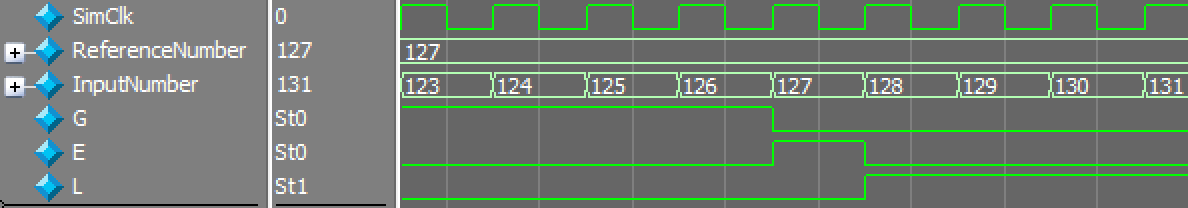
\includegraphics[width=.48\textwidth]{Images/ComparitorTestbench.png}
      \caption{Example output of testbench}
    \end{figure}

    %| Required Lab Demo
    %| =================================================================================================
    \demo{Comparitor}
      {Assign comparitor output to external LED module and use dipswitches for two four-bit inputs}
      {DE0-Nano configured with Comparitor}
      {Output LEDs will be inspected for proper operation as the student cycles through the inputs}

  %| =================================================================================================
  %| Lab Report
  %| =================================================================================================
  \section{Lab report}
    \IEEEPARstart{D}{ocumentation} is the most important part of an engineer's job. The sharper your writing skills the more employable you will be. Keep that in mind as you have to churn out documentation throughout college, it's not just busywork. This lab manual is written in almost textbook This particular lab report will require:
    \subsection{figures to include}
    \begin{itemize}
      \item Code listing of Full Adder
      \item Code listing for comparator
      \item It's important to remember Verilog is a Hardware Descriptive Language. The synthesis actually implements the Verilog in code. Quartus contains what are called \it{Netlist Viewers} that show the actual implementation. take a look at how Quartus synthesized your design as is shown in screencastX. Include screen captures of the combinatorial blocks listed in your design.
    \end{itemize}

    \subsection{Questions to Answer}
      \begin{enumerate}
        \item Do you think you would prefer the schematic design entry method of Lab two or the text based representation of this lab? In what situations do you think Schematic entry would be better, in which situations would Text base be advantageous.
      \end{enumerate}

  %| =================================================================================================
  %| Conclusion
  %| =================================================================================================
  \section{Conclusion}
    \IEEEPARstart{V}{erilog} is an IEEE standard(1364)\cite{Wikipedia:Verilog}, it is pervasive in industry and can be used to develop specialized hardware in the form of ASICs or reconfigurable FPGAs. It is important to underscore the differences between Verilog and a programming language like C, Java, even Assembly. Verilog offers the ability to take parallel action. Two numbers can be multiplied at once, multiple registers can be set and cleared. Entire microprocessors can be implemented on the Nano, FPGAs have become a valuable resource for a processor designer. The TerASIC documentation included with the DE0-Nano kit is pretty good and worth the read. It will help you get the most out of the development board. The CD included with the Nano will also include circuit schematics that can provide a great reference when it comes time to make one of your own.

  %| =================================================================================================
  %| Bibliography
  %| =================================================================================================
  \bibliographystyle{IEEEtran}
\bibliography{IEEEfull}


\end{document}